\documentclass[aspectratio=169,10pt]{beamer}
\usepackage[italian]{babel}
\usepackage[T1]{fontenc}
\usepackage[utf8]{inputenc}
\usepackage{pifont}
\usepackage{textcomp} % copyleft symbol con \textcopyleft
\usepackage{tikz}
\usetikzlibrary{backgrounds, fit, calc, positioning, arrows.meta, overlay-beamer-styles}
\PassOptionsToPackage{height=1cm}{beamerouterthemesidebar}
\usetheme{Berkeley}
\deftranslation[to=italian]{Definition}{Definizione}
\deftranslation[to=italian]{Example}{Esempio}

% !TeX spellcheck = it_IT

\title{Logica}
\author{Gianluca Amato}
\date{31 marzo 2023}

\newcommand{\xmark}{{\color{red}{\ding{55}}}}
\newcommand{\ra}{\rightarrow}
\newcommand{\conn}[1]{\textcolor{blue}{#1}}
\newcommand{\quant}[1]{\textcolor{blue}{#1}}
\newenvironment{inference}{\begin{tabular}{c}}{\end{tabular}}

\begin{document}

\begin{frame}
    \titlepage
    %\thanks{Rielaborazione delle slide di Gianluca Amato}
\end{frame}

\AtBeginSection[]
{
  \begin{frame}
  \frametitle{Contenuti}
   \tableofcontents[currentsection]
  \end{frame}
}

\section{Introduzione}

\begin{frame}{Cos'è la logica}
    \begin{definition}[Logica]
        La \alert{logica} (dal greco \textit{logos}, ovvero ``parola'', ``pensiero'') è lo studio del ragionamento.
    \end{definition}
    \begin{example}[Esempi di ragionamento]
        \begin{columns}
            \column{0.5\textwidth}
            \begin{center}
            Tutti gli uomini sono mortali.\\
            Socrate è un uomo.\\
            Dunque Socrate è mortale.\\[0.6cm]
            Ogni numero intero è o pari o dispari\\
            Il numero intero 3 non è pari\\
            Dunque 3 è dispari.
            \end{center}
            \column{0.5\textwidth}
            \centering
            
\includegraphics[width=2cm,keepaspectratio]{logica.png}

            \alert{Sono ragionamenti corretti?}
        \end{columns}
    \end{example}
    \begin{block}{Nota}
    Esistono varie forme di ragionamento, qui siamo interessati al \alert{ragionamento deduttivo}.
    \end{block}
\end{frame}

\subsection{Inferenze, proposizioni e connettivi}

\begin{frame}[label=inferenza]{Ragionamento deduttivo}
La forma principale del ragionamento deduttivo è quella dell'\alert{inferenza}.
\begin{definition}[Inferenza]
    Una \alert{inferenza} è una sequenza di \alert{proposizioni} di cui l'ultima è ottenuta come \alert{conclusione} delle rimanenti, che si assumono come \alert{premesse}.
\end{definition}
\begin{example}
\[
\begin{tikzpicture}
\tikzset{
    fillstyle/.style={rounded corners, draw=black},
    greenstyle/.style={fillstyle,fill=green!50},
    redstyle/.style={fillstyle,fill=red!50},
    bluestyle/.style={fillstyle,fill=blue!50},
    yellowstyle/.style={fillstyle,fill=yellow!50}
}
\clip (-6cm, -3cm) rectangle (6cm, 0.5cm);
\node (p1) {Tutti gli uomini sono mortali.};
\node (p2) [below of=p1] {Socrate è un uomo.};
\node (c) [below of=p2] {Socrate è mortale.};
\begin{scope}[on background layer]
\only<2->{\node (inf) [greenstyle, fit={(p1) (p2) (c)}, inner sep=0.5cm] {};}
\only<4->{\node (premises) [redstyle, fit={(p1) (p2)},  inner sep=0.2cm] {};}
\only<5->{\node (conclusion) [yellowstyle, fit={(c)},  inner sep=0.2cm] {};}
\only<3->{\node (prop1) [bluestyle, fit={(p1)},  inner sep=-0.05cm] {};}
\only<3->{\node (prop2) [bluestyle, fit={(p2)},  inner sep=-0.05cm] {};}
\only<3->{\node (prop3) [bluestyle, fit={(c)},  inner sep=-0.05cm] {};}
\end{scope}
\draw ($(c.west) + (-1cm,0.5cm)$) -- ($(c.east) + (1cm,0.5cm)$);
\only<2->{
    \draw (inf) ++ (-4.5cm,0cm)  node (inflabel) [greenstyle] {Inferenza};
    \draw [thick, ->] (inflabel) -- (inf.west);
}
\only<4->{
     \draw (premises) ++ (-4.5cm,0cm)  node (premiseslabel) [redstyle] {Premesse};
     \draw [thick, ->] (premiseslabel) -- (premises.west);
}
\only<5->{
     \draw (conclusion) ++ (-4.5cm,0cm)  node (conclusionlabel) [yellowstyle] {Conclusione};
     \draw [thick, ->] (conclusionlabel) -- (conclusion.west);
}
\only<3->{
    \draw (prop2) ++ (+4.5cm,0cm)  node (proplabel) [bluestyle] {Proposizioni};
    \draw [thick, ->] (proplabel) -- (prop1.east);
    \draw [thick, ->] (proplabel) -- (prop2.east);
    \draw [thick, ->] (proplabel) -- (prop3.east);
}
\end{tikzpicture}
\vspace{-0.4cm}
\]
\end{example}
\end{frame}

\begin{frame}{Proposizioni}
    \begin{definition}[Proposizione]
        Una \alert{proposizione} è una qualsiasi espressione linguistica per la quale ha senso chiedersi se sia vera o falsa.
    \end{definition}
    % \begin{columns}
    % \column{0.25\textwidth}
    %     \begin{center}
    %         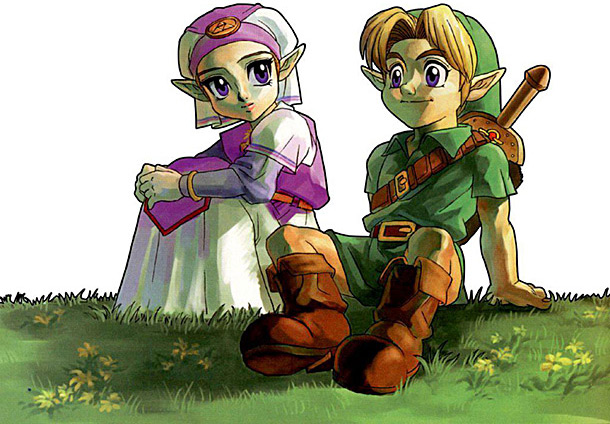
\includegraphics[width=3cm,keepaspectratio]{zelda.jpg}
    %     \end{center}
    % \column{0.7\textwidth}
    \begin{example}[Proposizioni \checkmark o no? \xmark]
        \begin{itemize}
            \item Link ama Zelda \only<1-4>{\makebox(0,0)[l]{\hspace{6cm}\vspace{-2.5cm}\raisebox{-1\totalheight}{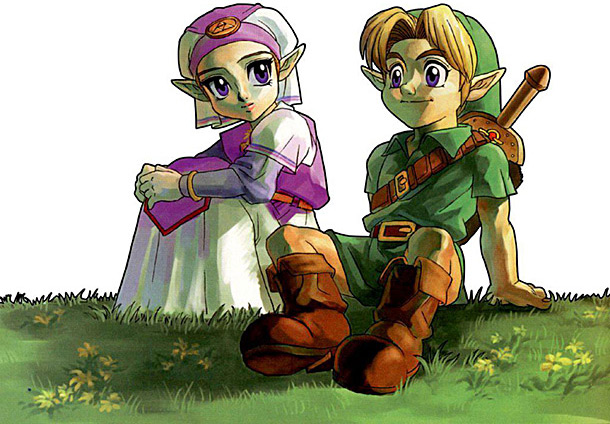
\includegraphics[width=4cm,keepaspectratio]{zelda.jpg}}}} \pause \checkmark
            \pause
            \item Link ama Zelda? \pause \xmark\ (è una \emph{domanda})
            \pause
            \item $4 + 2 = 6$
            \only<5-10>{\makebox(0,0)[l]{\hspace{7cm}\vspace{-1.5cm}\raisebox{-1\totalheight}{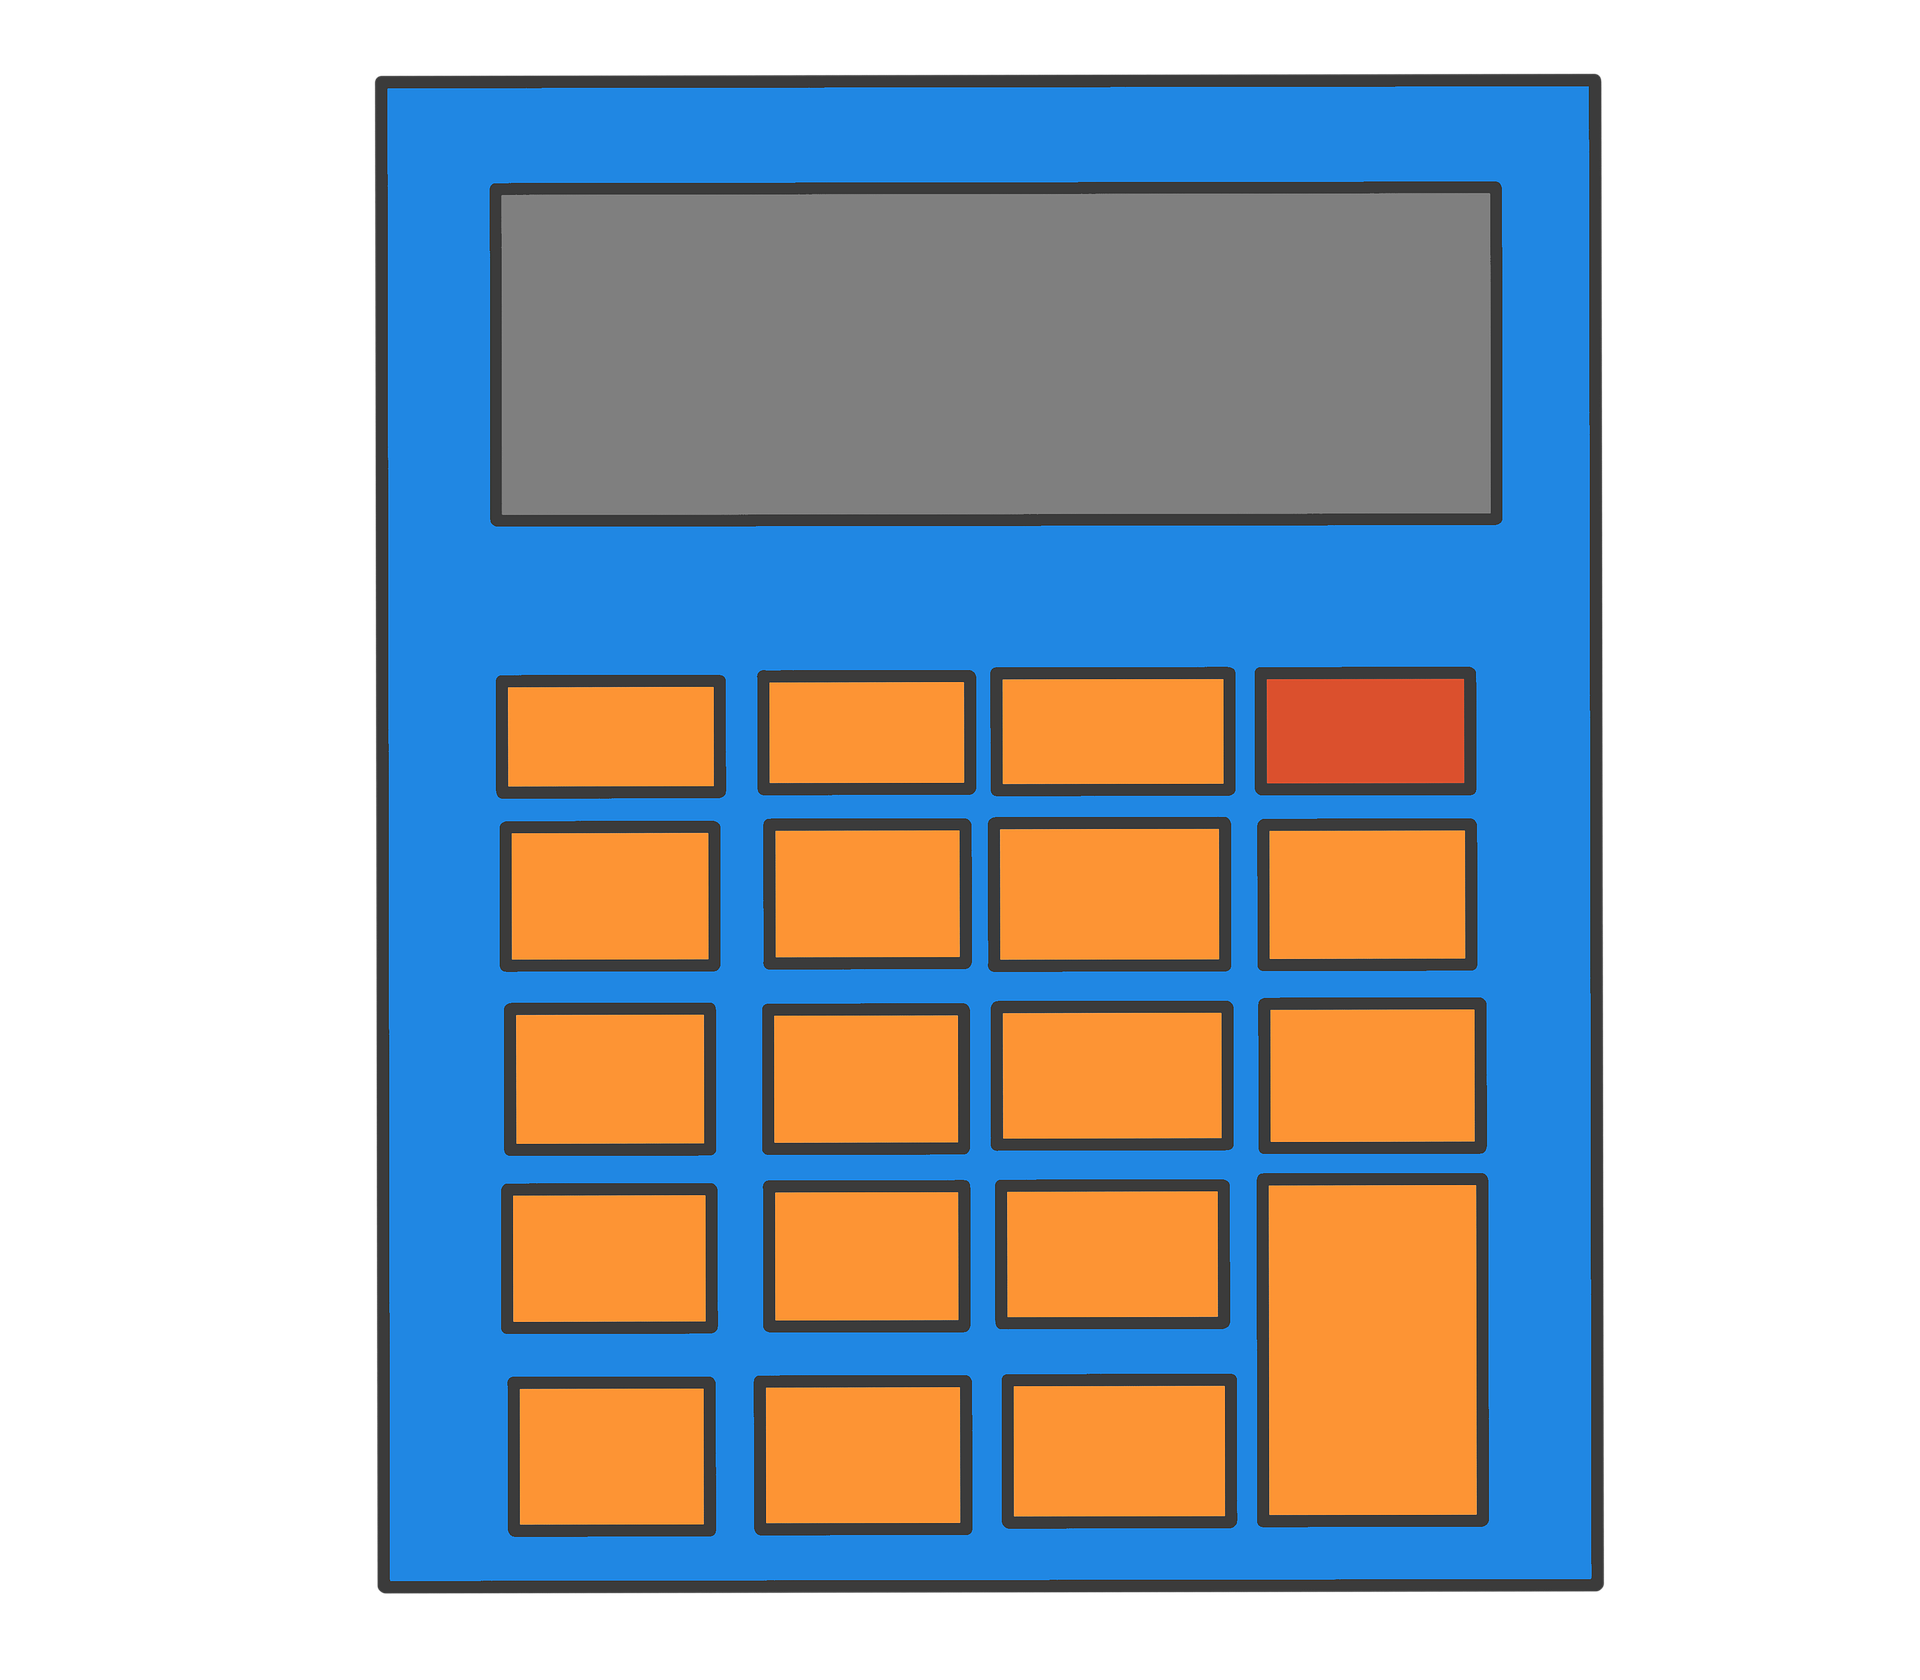
\includegraphics[width=3cm,keepaspectratio]{calcolatrice2.png}}}} \pause  \checkmark
            \pause
            \item $4 + 2 = 5$ \pause \checkmark (è falsa, ma è comunque una proposizione)
            \pause
            \item $3 + 5^2$ \pause \ \xmark \ (è una \emph{descrizione})
            \pause
            \item Tutti gli uomini sono mortali
            \only<11-12>{\makebox(0,0)[l]{\hspace{4cm}\vspace{1.5cm}\raisebox{-1\totalheight}{
\includegraphics[width=4cm,keepaspectratio]{mortal-kombat-11.jpg}}}}
            \pause \checkmark
            \pause
            \item Lazzaro, alzati e cammina!
            \only<13-14>{\makebox(0,0)[l]{\hspace{5cm}\vspace{2.5cm}\raisebox{-1\totalheight}{
\includegraphics[width=2.5cm,keepaspectratio]{lazzaro2.jpg}}}}
            \pause \xmark \ (è un \emph{ordine})
            \pause
            \item Quel ramo del lago di Como che volge a mezzogiorno
            \only<15-16>{\makebox(0,0)[l]{\hspace{1.3cm}\vspace{4.5cm}\raisebox{-1\totalheight}{
\includegraphics[width=2.3cm,keepaspectratio]{LagoDiComo.jpg}}}}
            \pause \xmark \ (è una \emph{descrizione})
        \end{itemize}
     \end{example}
    % \end{columns}
\end{frame}

\begin{frame}{Connettivi}
    \begin{columns}
            \column{0.65\textwidth}
            \begin{definition}[Connettivo]
                Un \alert{connettivo} è un elemento grammaticale che collega un certo numero di proposizioni tra di loro per formare una nuova proposizione.
            \end{definition}
            \column{0.3\textwidth}
            \begin{center}
                
\includegraphics[width=3cm,keepaspectratio]{puzzle.png}
            \end{center}
    \end{columns}
    \begin{example}
        \begin{itemize}
            \item Roma è la capitale d'Italia \conn{e} Lione è la capitale della Francia
            \item Roma è la capitale d'Italia \conn{oppure} Lione è la capitale della Francia
            \item \conn{Se} Roma è la capitale d'Italia \conn{allora} Lione è la capitale della Francia
            \item \conn{Non è vero} che Roma è la capitale d'Italia.
        \end{itemize}
    \end{example}
\end{frame}

\againframe<6>{inferenza}

\begin{frame}{Inferenze corrette}
	\begin{definition}[Inferenza corrette]
		Una inferenza è corretta se, ogni qualvolta le premesse sono vere, allora è necessariamente vera anche la conclusione.
  	\end{definition}
    \begin{example}[una inferenza corretta]
    \begin{center}
        \begin{inference}
        Carlo è ligure \conn{o} Stefano è piemontese\\
        Stefano \conn{non} è piemontese\\
        \hline
        Carlo è ligure
    \end{inference}
    \end{center}
    \end{example}
\end{frame}

\begin{frame}{Inferenze e forma logica}
	La correttezza di una inferenza dipende solo dalla \alert{forma logica} delle proposizioni.
	\begin{example}[inferenze con la stessa forma logica]
		\begin{center}
		\begin{inference}
			Carlo è ligure \conn{o} Stefano è piemontese\\
			Stefano \conn{non} è piemontese\\
			\hline
			Carlo è ligure
		\end{inference}
		\end{center}
        \medskip

        \begin{center}
		\begin{inference}
			Il maggiordomo è colpevole, \conn{oppure} la cameriera è colpevole.\\
			La cameriera \conn{non} è colpevole\\
			\hline
			Il maggiordomo è colpevole
		\end{inference}
        \end{center}
        \medskip

        \begin{center}
            \begin{inference}
		\conn{O} due buchi neri si sono scontrati \conn{oppure} il rivelatore di onde gravitazionali è rotto.\\
		Il rivelatore di onde gravitazionali \conn{non} è rotto.\\
        \hline
         Due buchi neri si sono scontrati.
       \end{inference}
       \end{center}
	\end{example}
\end{frame}

\begin{frame}{Regole di inferenza}
	Mettiamo in evidenza la \alert{forma logica} dell'inferenza.\\
    \medskip
    Usiamo delle \alert{lettere proposizionali}, al posto delle proposizioni:
	\begin{center}
		A  = ``Carlo è ligure'' \hspace{1cm} B = ``Stefano è piemontese''
	\end{center}
	otteniamo
	\[
	\begin{tikzpicture}[remember picture]
	\node (carlo) {\begin{inference}
		Carlo è ligure \conn{o} Stefano è piemontese\\
		Stefano \conn{non} è piemontese\\
		\hline
		Carlo è ligure
	\end{inference}
	};
	\node (disj) [right=of carlo] {
		\begin{inference}
		A o B\\
		non B\\
		\hline
		A
		\end{inference}
	};
	\draw [-{Latex[width=3mm]},very thick] (carlo) -- (disj);
	\end{tikzpicture}
	\]
	\pause
	\begin{definition}[Regola di inferenza]
		Una inferenza in cui usiamo \alert{lettere proposizionali}  invece di proposizioni vere e proprie prende il nome di \alert{regola di inferenza}.
		\begin{tikzpicture}[overlay, remember picture]
		\draw [red, thick] (disj) circle (1cm);
		\path (disj) ++ (0,-1.3cm) node [red] {Regola di inferenza};
		\end{tikzpicture}
	\end{definition}
\end{frame}

\subsection{Regole di inferenza corrette}

\begin{frame}{Regole di inferenza corrette}
	Se al contrario rimpiazziamo le lettere con delle proposizioni, troviamo una \alert{istanza} della regola.
    Se una regola è corretta, tutte le istanze lo sono.

    \begin{example}[Sillogismo disgiuntivo]
        La regola di inferenza\\
            \begin{center}
        	\begin{inference}
            A o B\\
            non B\\
            \hline
            A
        \end{inference}
        \end{center}
        chiamata \alert{regola del sillogismo disgiuntivo} è corretta, quindi\\
        \begin{center}
        		\begin{inference}
            Il maggiordomo è colpevole, \conn{oppure} la cameriera è colpevole.\\
            La cameriera \conn{non} è colpevole\\
            \hline
            Il maggiordomo è colpevole
        \end{inference}\\
        \end{center}
        è corretta.
    \end{example}
\end{frame}

\begin{frame}{Un'altra regola corretta: modus ponens}
	Consideriamo l'inferenza
	\begin{center}
		\begin{inference}
			\conn{Se} Fabio è genovese, \conn{allora} Fabio è ligure\\
			Fabio è genovese\\
			\hline
			Fabio è ligure
		\end{inference}
	\end{center}
        \only<1-1>{\makebox(0,0)[l]{\hspace{3cm}\vspace{-2.5cm}\raisebox{-1\totalheight}{
\includegraphics[width=8.5cm,keepaspectratio]{cartina_liguria.png}}}}
	\pause
	Si generalizza nella regola:
	\begin{center}
		\begin{inference}
			Se A allora B\\
			A\\
			\hline
			B
		\end{inference}
	\end{center}
	detta \alert{regola del modus ponens}. Vedi anche:
	\begin{center}
		\begin{inference}
			\conn{Se} sono colpevole \conn{allora} devo essere punito\\
			Sono colpevole\\
			\hline
			Devo essere punito
		\end{inference}
	\end{center}
\end{frame}

\begin{frame}{Un'altra regola corretta: modus tollens}
	Consideriamo l'inferenza
	\begin{center}
		\begin{inference}
			\conn{Se} Fabio è genovese, \conn{allora} Fabio è ligure\\
			Fabio \conn{non} è ligure\\
			\hline
			Fabio \conn{non} è genovese
		\end{inference}
	\end{center}
	\pause
	Si generalizza nella regola:
	\begin{center}
		\begin{inference}
			Se A allora B\\
			non B\\
			\hline
			non A
		\end{inference}
	\end{center}
	detta \alert{regola del modus tollens}. Vedi anche:
	\begin{center}
		\begin{inference}
			\conn{Se} sono colpevole \conn{allora} devo essere punito\\
			\conn{Non} devo essere punito\\
			\hline
			\conn{Non} sono colpevole
		\end{inference}
	\end{center}
\end{frame}

\subsection{Regole di inferenza non corrette}

\begin{frame}{Fallacia della negazione dell'antecedente (1)}
	Consideriamo l'inferenza
	\begin{center}
		\begin{inference}
			\conn{Se} sono un ladro \conn{allora} devo essere punito\\
			\conn{Non} sono un ladro\\
			\hline
			Non devo essere punito
		\end{inference}
	\end{center}
         \only<1-1>{\makebox(0,0)[l]{\hspace{5cm}\vspace{-3.5cm}\raisebox{-1\totalheight}{
\includegraphics[width=4.5cm,keepaspectratio]{lupin.png}}}}
	\pause
    che si generalizza nella regola
    \begin{center}
        \begin{inference}
            Se A allora B\\
            non A\\
            \hline
            non B
        \end{inference}
    \end{center}
	È corretta?
\end{frame}

\begin{frame}{Fallacia della negazione dell'antecedente (2)}
   All'apparenza lo sembra, ma consideriamo un'altra istanza della regola.
   \begin{center}
   \begin{inference}
        \conn{Se} Fabio è pescarese, \conn{allora} Fabio è abruzzese \only<3->{\checkmark}\\
        Fabio \conn{non} è pescarese \only<4->{\checkmark}\\
        \hline
        Fabio \conn{non} è abruzzese \only<5->{\xmark}
    \end{inference}
   \end{center}
   È corretta?
         \only<1-1>{\makebox(0,0)[l]{\hspace{5cm}\vspace{-3.5cm}\raisebox{-1\totalheight}{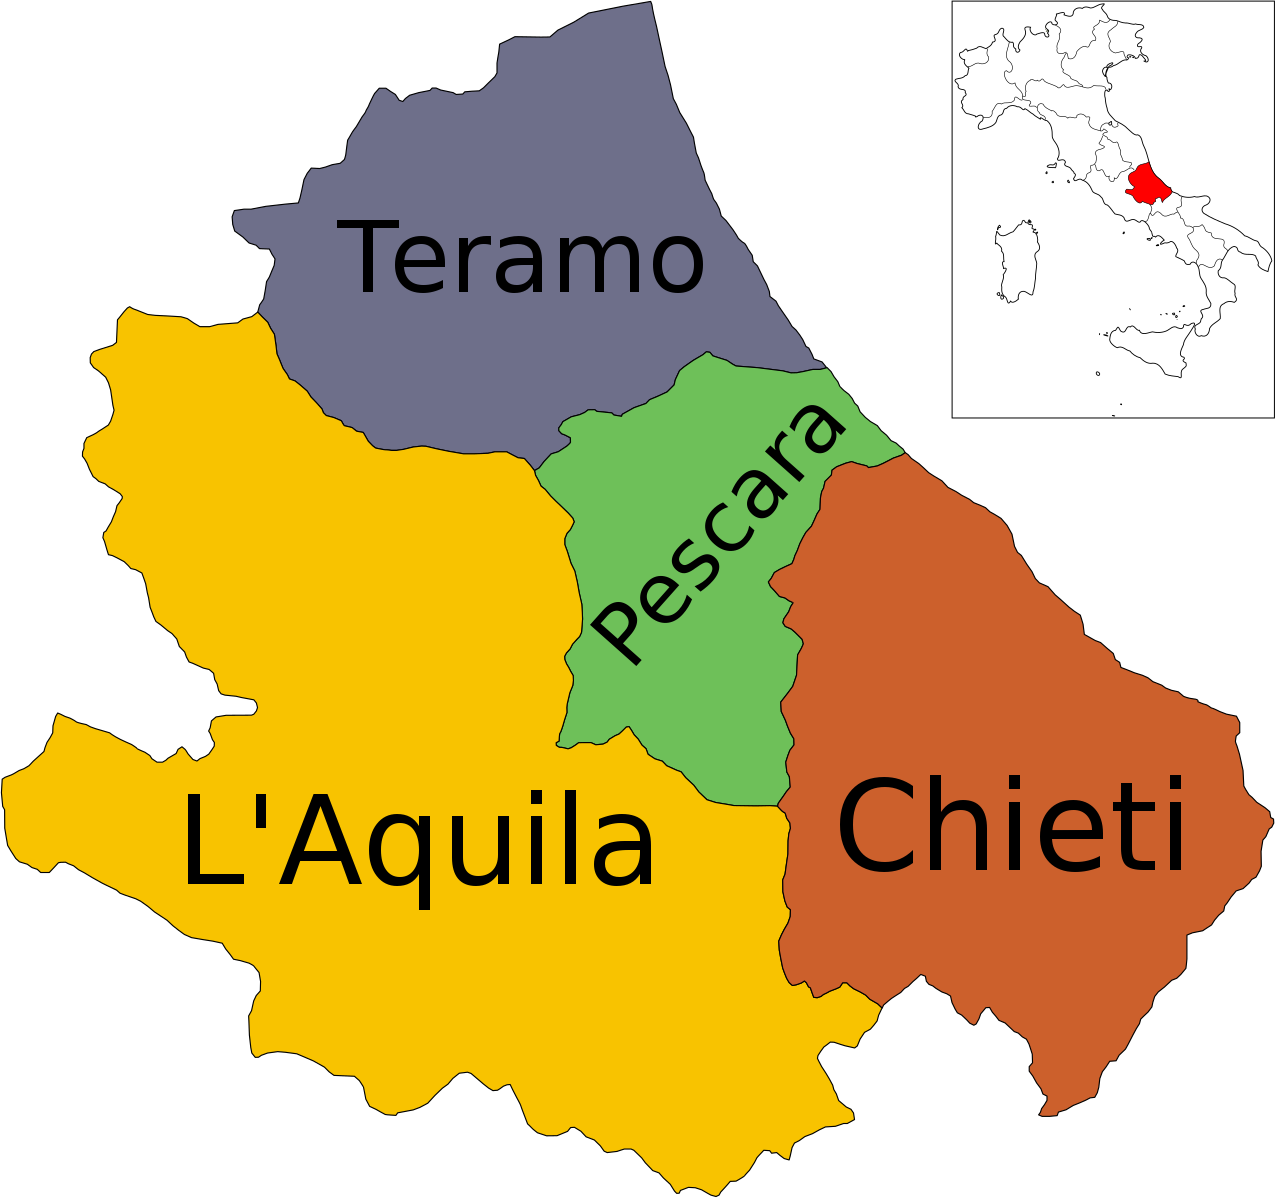
\includegraphics[width=4.5cm,keepaspectratio]{abruzzo.png}}}}

   \pause
   \medskip
   Questa regola \textbf{non è} corretta: pensate al caso in cui Fabio sia nato a Chieti.

   \onslide<6->{\medskip
       Abbiamo trovato un \alert{controesempio}. L'inferenza non è corretta.}

   \onslide<7->{\medskip
       Ed infatti, se ci pensiamo bene, non è corretta neanche la prima regola di inferenza: magari non sono un ladro, ma devo essere punito per qualche altro motivo.}
\end{frame}

\begin{frame}{Fallacia dell'affermazione del conseguente}

	Consideriamo questa inferenza\ldots
	\begin{center}
		\begin{inference}
 		    \conn{Se} sono un ladro \conn{allora} devo essere punito\\
			Devo essere punito\\
			\hline
			Sono un ladro
	\end{inference}
	\end{center}
	\pause
    che si generalizza nella regola
    \begin{center}
        \begin{inference}
            Se A allora B\\
            B\\
            \hline
            A
        \end{inference}
    \end{center}
	e questa\ldots
	\begin{center}
		\begin{inference}
			\conn{Se} Fabio è pescarese, \conn{allora} Fabio è abruzzese\\
			Fabio è abruzzese\\
			\hline
			Fabio è pescarese
		\end{inference}
	\end{center}
	\pause
    Anche se la prima può sembrarci corretta (ma non lo è, potrei dover essere punito per qualche altro motivo), la regola di inferenza
    \alert{non è corretta}.
\end{frame}

\begin{frame}{Correttezza delle inferenze e delle conclusioni}
    \begin{block}{Attenzione!}
    Se le premesse di una inferenza sono false, anche la conclusione può essere falsa, sebbene l'inferenza sia corretta.
    \end{block}

   Abbiamo detto che il \alert{modus ponens} è corretto:
    \begin{center}
        \begin{inference}
        Se A allora B\\
        A\\
        \hline
        B
        \end{inference}
    \end{center}
    Ma guardiamo questa istanza:
    \begin{center}
        \begin{inference}
        \conn{Se} Napoleone è francese \conn{allora} Napoleone è abruzzese\\
        Napoleone è francese\\
        \hline
        Napoleone è abruzzese
        \end{inference}
    \end{center}
\end{frame}

% \begin{frame}{Premesse incosistenti}
%     \begin{center}
%         \begin{inference}
%         A\\
%         non A\\
%         \hline
%         B
%         \end{inference}
%     \end{center}
%     Questa inferenza vuol dire che se ``A'' è vero, ma nello stesso tempo ``non A'' è vero (quindi ``A'' è falso) allora possiamo inferire una qualunque proposizione B.

%     \medskip
%     In latino si usa talvolta dire \emph{ex falso quodlibet}, dal falso segue qualsiasi cosa.
% \end{frame}


\begin{frame}<presentation:0>{Regole di inferenza a livello predicativo}
	Negli esempi visti prima, le regole di inferenza sono a livello \alert{proposizionale}: la loro verità dipende dai legami tra le proposizioni.

    \medskip
    Queste inferenze sono più complesse:
	\begin{center}
		\begin{inference}
			2 è minore di 5\\
			Se un numero è minore di un altro, allora il secondo è maggiore del primo\\
			\hline
			5 è maggiore di 2
		\end{inference}

		\medskip\medskip
		\begin{inference}
		La retta $r$ è perpendicolare alla retta $s$\\
		Se una retta è perpendicolare a un'altra, la seconda interseca la prima\\
		\hline
		$s$ interseca $r$
		\end{inference}

		\medskip\medskip
		\begin{inference}
		Maria è moglie di Aldo\\
		Se una persona è moglie di un'altra, allora quest'ultima è marito della prima\\
		\hline
		Aldo è marito di Maria
		\end{inference}
	\end{center}
	Hanno la stessa \alert{forma logica}.
\end{frame}

\newcommand{\myfbox}[2]{\tikz[baseline=(n.base)]\node(n)[alt=<1>{fill=#1!50}]{#2};}
\newcommand{\myfboxbis}[2]{\tikz[baseline=(n.base)]\node(n)[alt=<2>{fill=#1!50}]{#2};}

\begin{frame}<presentation:0>{Evidenziare la forma logica}
	\tikzstyle{every node} = [rounded corners, outer sep=0, inner sep=0.1cm]
	\begin{center}
			\begin{inference}
				\myfbox{red}{2}\myfbox{green}{è minore di}\myfbox{blue}{5}\\
				Se\myfbox{orange}{un numero}\myfbox{green}{è minore di}\myfbox{pink}{un altro}, allora\myfbox{pink}{il secondo}\myfbox{gray}{è maggiore del} \myfbox{orange}{primo}\\
				\hline
				\myfbox{blue}{5}\myfbox{gray}{è maggiore di}\myfbox{red}{2}
			\end{inference}\\[0.2cm]
		$\Downarrow$\\[0.2cm]
		\begin{inference}
			\myfbox{green}{R}\myfbox{red}{a}\myfbox{blue}{b}\\
			\myfboxbis{green}{per ogni }\myfbox{orange}{$x$}, \myfboxbis{green}{per ogni } \myfbox{pink}{$y$}, \myfboxbis{red}{se} \myfbox{green}{R}\myfbox{orange}{$x$}\myfbox{pink}{$y$}\myfboxbis{red}{allora}\myfbox{gray}{S}\myfbox{pink}{$y$}\myfbox{orange}{$x$}\\
			\hline
			\myfbox{gray}{S}\myfbox{blue}{b}\myfbox{red}{a}\\
		\end{inference}\\[0.2cm]
		\only<2->{
		$\Downarrow$\\[0.2cm]
		\begin{inference}
			Rab\\
			$\myfboxbis{green}{$\forall x \forall y$} (Rxy \myfboxbis{red}{$\ra$} Syx)$\\
			\hline
			Sba
		\end{inference}
	}
	\end{center}
\end{frame}

\begin{frame}{Regole di inferenza con i quantificatori}
	\tikzstyle{every node} = [rounded corners, outer sep=0, inner sep=0.1cm]

	Negli esempi visti prima, le regole di inferenza sono a livello \alert{proposizionale}: la loro verità dipende dai legami tra le proposizioni.

	\medskip
	Queste inferenze sono più complesse:
	\begin{center}
		\begin{inference}
			\myfbox{red}{Napoleone} \myfbox{green}{è corso}\\
			Tutti \myfbox{green}{i corsi}  \myfbox{gray}{sono francesi}\\
			\hline
			\myfbox{red}{Napoleone} \myfbox{gray}{è francese}
		\end{inference}
		\qquad
		\begin{inference}
           	\myfbox{red}{Socrate} \myfbox{green}{è un uomo}\\
			Tutti \myfbox{green}{gli uomini}  \myfbox{gray}{sono mortali}\\
			\hline
			\myfbox{red}{Socrate} \myfbox{gray}{è mortale}
		\end{inference}
	\end{center}
	ma hanno la stessa \alert{forma logica} e corrispondono alla regola
	\begin{center}
		\begin{inference}
		$\myfbox{green}{P} \myfbox{red}{(a)}$\\
		\conn{per ogni} $x$, \conn{se} $\myfbox{green}{P}(x)$ \conn{allora} $\myfbox{gray}{Q}(x)$\\
		\hline
		$\myfbox{gray}{Q}  \myfbox{red}{(a)}$
	\end{inference}
	\end{center}
\end{frame}

\section{Logica delle proposizioni}

\subsection{Negazione}

\begin{frame}{Negazione}
    La \alert{negazione} trasforma una proposizione vera in una falsa e viceversa.
    \medskip

    In italiano è di solito resa con:
    \begin{itemize}
        \item \conn{non è vero che} prima della proposizione da negare
        \item \conn{non} prima del verbo della proposizione da negare
    \end{itemize}
    \begin{example}
        Roma è la capitale d'Italia (\checkmark) \pause
        \begin{itemize}
            \item \conn{Non è vero che} Roma è la capitale d'Italia (\xmark)
            \item  Roma \conn{non} è la capitale d'Italia (\xmark)
        \end{itemize}
        \medskip

        \pause
        Dante Alighieri ha scritto ``I Promessi Sposi'' (\xmark) \pause
        \begin{itemize}
            \item \conn{Non è vero che} Dante Alighieri ha scritto ``I Promessi Sposi'' (\checkmark)
            \item  Dante Alighieri \conn{non} ha scritto ``I Promessi Sposi'' (\checkmark)
        \end{itemize}
    \end{example}
\end{frame}

\subsection{Congiunzione}

\begin{frame}{Congiunzione}
    La \alert{congiunzione} collega due proposizioni tra di loro. La nuova proposizione risultante è vera quando entrambe le proposizioni di partenza sono vere. \medskip

    In italiano è di solito resa con \conn{e} oppure \conn{ma}.
    \begin{example}
        Roma è la capitale d'Italia (\checkmark) \\
        Parigi è la capitale della Francia (\checkmark) \pause
        \begin{itemize}
            \item Roma è la capitale d'Italia \conn{e} Parigi è la capitale della Francia (\checkmark)
            \item Roma è la capitale d'Italia \conn{ma} Parigi è la capitale della Francia (\checkmark)
        \end{itemize}
        \medskip

        \pause
        $2+2 = 4$ (\checkmark) \\
        $3 \times 2= 5$  (\xmark) \pause
        \begin{itemize}
            \item $2+2 = 4$ \conn{e} $3 \times  2= 5$  (\xmark)
        \end{itemize}
    \end{example}
\end{frame}

\begin{frame}{Congiunzione nella lingua italiana}
    Talvolta in italiano si cerca di evitare le ripetizioni, e il connettivo \conn{e} non si trova più tra due proposizioni.

    \begin{example}
        Carlo \conn{e} Maria sono appassionati di baseball \medskip

        \hspace{2cm} è una abbreviazione di\medskip

        Carlo è appassionato di baseball \conn{e} Maria è appassionata di baseball
    \end{example}

    \pause
    Ma attenzione!!! Non tutte le \conn{e} sono istanze della congiunzione
    \begin{example}
        Carlo e Maria sono amici\medskip

        \hspace{2cm} \textbf{non è} una abbreviazione di\medskip

        Carlo è amico \conn{e} Maria è amica\medskip
    \end{example}
\end{frame}

\subsection{Disgiunzione}

\begin{frame}{Disgiunzione}
    La \alert{disgiunzione} collega due proposizioni tra di loro. La nuova proposizione risultante è vera quando \textbf{una} delle proposizioni di partenza è vera. \medskip

    In italiano è di solito resa con \conn{o} ed \conn{oppure}.
    \begin{example}
        Roma è la capitale d'Italia (\checkmark)\\
        Lione è la capitale della Francia (\xmark)\\
        \pause
        \begin{itemize}
            \item Roma è la capitale d'Italia \conn{o} Lione è la capitale della Francia (\checkmark)
            \item Roma è la capitale d'Italia \conn{oppure} Lione è la capitale della Francia (\checkmark)
            \item \conn{O} Roma è la capitale d'Italia \conn{oppure} Lione è la capitale della Francia (\checkmark)
        \end{itemize}
        \medskip

        \pause
        $2+2 = 5$ (\xmark) \\
        $3 \times 2= 7$  (\xmark) \pause
        \begin{itemize}
            \item  $2+2 = 5$ \conn{oppure} $3 \times 2= 7$  (\xmark)
        \end{itemize}
    \end{example}
\end{frame}

% \begin{frame}{Disgiunzione 2}
%     \begin{block}{Uso nella lingua italiana}
%     Riconsideriamo l'esempio di prima:\\
%     \begin{itemize}
%     \item Roma è la capitale d'Italia \alert{o} Parigi è la capitale della Francia
%     \end{itemize}
%     \medskip
%     È una frase piuttosto strana:
%     \begin{itemize}
%     \item difficilmente la sentiremmo dire nella vita di tutti i giorni;
%     \item se la pronunciassimo durante una interrogazione il prof. potrebbe anche esser tentato di correggerci
%     \begin{itemize}
%         \item \guillemotleft Carlo, dovresti dire ``Roma è la capitale d'Italia \alert{e} Parigi è la capitale della Francia'' \guillemotright
%         \item ma la nostra affermazione è vera, semmai non è molto precisa
%     \end{itemize}
%     \end{itemize}
%     \end{block}
% \end{frame}

\begin{frame}{Disgiunzione nella lingua italiana}
    Riconsideriamo l'esempio di prima:\\
    \begin{example}
    Roma è la capitale d'Italia \conn{o} Lione è la capitale della Francia
    \end{example}
    È una proposizione piuttosto strana. Nella lingua italiana, utilizziamo la disgiunzione quasi sempre quando le due proposizioni sono strettamente correlate tra di loro. Ad una interrogazione, uno studente un po' ignorante potrebbe rispondere:
    \begin{example}
    Roma è la capitale d'Italia \conn{o} Milano è la capitale d'Italia
    \end{example}
    Spesso, in questi casi, abbreviamo la frase, come già visto per la congiunzione
    \begin{example}
    Roma \conn{o} Milano è la capitale d'Italia
    \end{example}
\end{frame}

\begin{frame}{Disgiunzione inclusiva ed esclusiva}
    Consideriamo ancora una proposizione un po' innaturale:
    \begin{example}
    Roma è la capitale d'Italia \conn{o} Parigi è la capitale della Francia
    \end{example}
    Cosa ne pensate ? È vera o falsa ?
    \pause
    \begin{itemize}
    \item se per voi la frase è \textbf{vera}, vuol dire che considerate la ``\conn{o}'' in senso \alert{inclusivo}
    \begin{itemize}
    \item se entrambe le proposizioni di base sono vere, la disgiunzione è vera;
    \item la disgiunzione inclusiva è vera quando \alert{una o più} delle proposizioni di base è vera;
    \end{itemize}
    \pause
    \item se per voi la frase è \textbf{falsa}, vuol dire che considerate la ``\conn{o}'' in  senso \alert{esclusivo}
    \begin{itemize}
        \item se entrambe le proposizioni di base sono vere, la disgiunzione è falsa;
        \item per voi la ``\conn{o}'' introduce una alternativa tra due possibilità, una delle quali deve essere falsa;
        \item la disgiunzione esclusiva è vera quando \alert{esattamente una} delle proposizioni di base è vera.
    \end{itemize}
    \end{itemize}
\end{frame}


\begin{frame}{Disgiunzione inclusiva ed esclusiva}
    Abbiamo detto prima
    \begin{definition}
    La \alert{disgiunzione} collega due proposizioni tra di loro. La nuova proposizione risultante è vera quando \textbf{una} delle proposizioni di partenza è vera.
    \end{definition}
    In realtà siamo stati imprecisi. Dovremmo dire:
        \begin{definition}[Disgiunzione inclusiva]
            La \alert{disgiunzione inclusiva} collega due proposizioni tra di loro. La nuova proposizione risultante è vera quando \textbf{almeno una} delle proposizioni di partenza è vera.
    \end{definition}
    e
    \begin{definition}[Disgiunzione esclusiva]
            La \alert{disgiunzione esclusiva} collega due proposizioni tra di loro. La nuova proposizione risultante è vera quando \textbf{esattamente una} delle proposizioni di partenza è vera.
    \end{definition}
\end{frame}

\begin{frame}{Disgiunzione inclusiva ed esclusiva nella lingua italiana 1}
    Ma chi ha ragione ? La ``\conn{o}'' in italiano è inclusiva od esclusiva ?
    \medskip

    Spesso il problema non si pone perché, dal contesto, sappiamo che le due proposizioni non possono essere entrambe vere.
    \pause

    \begin{example}
        Vi assicuro che la seguente proposizione è vera:
        \begin{itemize}
        \item La capitale della California è Sacramento \conn{o} Los Angeles.
        \end{itemize}
        Vuol dire che possono essere entrambe capitali ?
    \end{example}
    \pause
         Ovviamente no, perché sappiamo che uno stato non può avere due capitali, ma se questa  ``impossibilità'' dettata dal contesto non si verifica, l'italiano è molto ambiguo.
    \begin{example}
        Vi assicuro che la seguente proposizione è vera:
        \begin{itemize}
        \item La bandiera della California contiene una stella \conn{o} un orso.
        \end{itemize}
        Vuol dire che la bandiera può avere entrambe ?
    \end{example}
\end{frame}

\begin{frame}{Disgiunzione inclusiva ed esclusiva nella lingua italiana 2}
    In generale, nella lingua di tutti i giorni, non è chiaro se ``\conn{o}''  e ``\conn{oppure}'' vadano intesi in senso inclusivo o esclusivo, ma
    \begin{block}{Osservazione finale}
    \begin{itemize}
        \item quando si studia logica (quindi anche negli esercizi) lo si intende sempre inclusivo;
        \item in matematica è sempre inclusivo:
        \begin{itemize}
        \item la proposizione ``$2 + 2 = 4$ \conn{oppure} $5$ è dispari'' è vera!
        \end{itemize}
    \end{itemize}
    \end{block}
\end{frame}

\begin{frame}{Approfondimento: tavole di verità}
    Si può descrivere il comportamento dei connettivi con le \alert{tavole di verità}.

    \begin{example}[Tavole di verità dei connettivi]
        Indichiamo con $P$, $Q$, \ldots delle proposizioni qualunque. Allora:
        \begin{center}
            \begin{tabular}[t]{c|c}
                $P$ & non $P$ \\
                \hline
                V & F       \\
                F & V
            \end{tabular}
            \hspace{2cm}
            \begin{tabular}[t]{c|c|c}
                $P$ & $Q$ & $P$ e $Q$ \\
                \hline
                F & F & F\\
                F & V & F\\
                V & F & F\\
                V & V & V\\
            \end{tabular}
            \hspace{2cm}
            \begin{tabular}[t]{c|c|c}
                $P$ & $Q$ & $P$ o $Q$ \\
                \hline
                F & F & F\\
                F & V & V\\
                V & F & V\\
                V & V & V\\
            \end{tabular}
        \end{center}
    \end{example}
    \begin{block}{Nota}
        Venite dall'ITIS e avete studiato le \alert{porte logiche} ? Noterete allora che i connettivi sono praticamente la stessa cosa delle porte logiche \texttt{not}, \texttt{and} e \texttt{or}.
    \end{block}
\end{frame}

\begin{frame}{Approfondimento: simboli matematici per i connettivi}
    Ai matematici piacciono i simboli:
    \begin{definition}[Simboli dei connettivi]
        \begin{itemize}
            \item negazione (non $P$):  $\neg P$
            \item congiunzione ($P$ e $Q$):  $P \wedge Q$
            \item disgiunzione ($P$ o $Q$):  $P \vee Q$

        \end{itemize}
    \end{definition}
    \begin{example}
        $2 + 2 = 4$ \conn{e} $3 \times 2 = 6$\medskip

        \hspace{2cm}$\Downarrow$ usando i simboli visti sopra \medskip

        $2 + 2 = 4 \wedge 3 \times 2 = 6$
    \end{example}
\end{frame}

\begin{frame}{Approfondimento: forme proposizionali}
   Usando le lettere $P$, $Q$, $R$ etc... e i simboli $\wedge$, $\vee$ e $\neg$ è possibile costruire delle \alert{formule logiche}, chiamate anche \alert{forme proposizionali}.
   \begin{example}
   $P \vee \neg (Q \wedge R)$ è una forma proposizionale.
   \end{example}
   \pause
   Una forma proposizionale è quella che abbiamo precedentemente chiamato \alert{forma logica}:
   \begin{example}[dalle forme proposizionali alle proposizioni]
       Considerate la forma proposizionale  $P \wedge \neg (Q \wedge R)$. Allora se
       \begin{itemize}
       \item $P={}$ Il maggiordomo è l'assassino
       \item $Q={}$ Il delitto è stato commesso in casa
       \item $R={}$ Il coltello è l'arma del delitto
       \end{itemize}
       otteniamo
       \begin{itemize}
           \item Il maggiordomo è l'assassino \conn{o} \conn{non è vero che} il delitto è stato commesso in casa \conn{con} il coltello.
       \end{itemize}
   \end{example}
\end{frame}

\subsection{Implicazione}

\begin{frame}{Implicazione}
    L'\alert{implicazione} collega due proposizioni $P$ e $Q$ tra di loro, e viene di solito resa in italiano con  ``\conn{se} $P$ \conn{allora} $Q$''.    \begin{itemize}
        \item $P$ è chiamato \alert{antecedente};
        \item $Q$ è chiamato \alert{conseguente}.
    \end{itemize}
    L'implicazione è sempre vera, tranne quando l'antecedente è vero e il conseguente è falso.
    \begin{example}[Vero o falso?]
        \begin{itemize}
            \item \conn{se} Roma è la capitale d'Italia \conn{allora} 3+2=5 \pause (\checkmark)
            \pause
            \item \conn{se} Roma è la capitale d'Italia \conn{allora} 3+2=0 \pause (\xmark)
            \pause
            \item \conn{se} gli elefanti volano \conn{allora} 3+2=5 \pause (\checkmark)
            \pause
            \item \conn{se} gli elefanti volano \conn{allora} 3+2=0 \pause (\checkmark)
        \end{itemize}
    \end{example}
\end{frame}

\begin{frame}[fragile]{Implicazione e linguaggio naturale}
    Gli esempi di prima vi sono sembrati strani ?
    \begin{block}{Note}
        Quello che vi sto presentando è solo un tipo particolare di logica, chiamata \alert{logica classica proposizionale}. Il \conn{se \ldots allora} in italiano non è quasi mai corrispondente alla implicazione di questa logica.
    \end{block}
    \begin{example}
        \begin{itemize}
        \item \conn{se} sarai promosso a scuola, \conn{allora} ti comprerò la PlayStation 5
        \begin{itemize}
            \item coinvolge azioni che avverranno in futuro, non ora: è il reame della \alert{logica temporale};
            \item la versione classica proposizionale  sarebbe:\\
            ``\conn{se} sei stato promosso a scuola, \conn{allora} ti ho comprato la PlayStation 5''  \raisebox{-0.2\totalheight}{
\includegraphics[width=0.5cm,keepaspectratio]{vomitosa.png}}
        \end{itemize}
        \pause
        % \item \conn{se} un oggetto viene lanciato da una torre, \conn{allora} cade a terra
        % \begin{itemize}
        %     \item ``un oggetto viene lanciato da una torre'' non è un proposizione, perché non sta parlando né di un oggetto né di un momento specifico, è una affermazione ipotetica;
        %     \item quello che intendiamo dire è che in ogni situazione possibile in cui un oggetto viene lanciato, necessariamente questo cadrà per terra;
        %     \item necessità e possibilità sono il reame della \alert{logica modale}.
        % \end{itemize}
        \item \conn{se} $n$ è divisibile per $4$ \conn{allora} $n$ è pari
        \begin{itemize}
            \item $n$ è divisibile per $4$ non è una proposizione, non possiamo dire se è vera è falsa perché ciò dipende dal valore di $n$: siamo nel reame della \alert{logica dei predicati};
            \item la versione proposizionale sarebbe ``\conn{se} 8 è divisibile per $4$ \conn{allora} $8$ è pari'' \raisebox{-0.2\totalheight}{
\includegraphics[width=0.5cm,keepaspectratio]{vomitosa.png}}
            \item si potrebbe trovare forse in un testo matematico, ma non è certo così comune.
        \end{itemize}
        \end{itemize}
    \end{example}
\end{frame}

\subsection{Inferenze ed equivalenze logiche}

\begin{frame}{Equivalenze logiche}
    \begin{definition}
    Due proposizioni sono \alert{logicamente equivalenti} quando hanno sempre lo stesso valore di verità, indipendentemente dai valori di verità delle proposizioni semplici che la compongono.
    \end{definition}
    \begin{columns}
        \column{0.65\textwidth}
     \begin{example}[Commutatività della congiunzione]
        \emph{Pikachu è giallo \conn{e} Bulbasaur è verde} [\alert{$P \wedge Q$}]\medskip\\
        \hspace{1cm} è equivalente a  (si usa il simbolo $\equiv$)\medskip\\
        \emph{Bulbasaur è verde \conn{e} Pikachu è giallo} [\alert{$Q \wedge P$}]
     \end{example}
     \begin{example}[Idempotenza della congiunzione]
        \emph{Pikachu è giallo \conn{e} Pikachu è giallo}  [\alert{$P \wedge P$}]\medskip\\
        \hspace{1cm}$\equiv$\medskip\\
        \emph{Pikachu è giallo}  [\alert{$P$}].
     \end{example}
       \column{0.3\textwidth}
            \begin{center}
                
\includegraphics[width=2cm,keepaspectratio]{Pikachu.png}

                
\includegraphics[width=2cm,keepaspectratio]{Bulbasaur.png}
            \end{center}
    \end{columns}
\end{frame}

\begin{frame}{Equivalenze logiche notevoli 1}
Alcune equivalenze logiche sono molto importanti. Tra di queste:
\begin{example}[Doppia negazione]
\conn{Non è vero che} Pikachu \conn{non} è giallo [\alert{$\neg \neg P$}]\\
\medskip
\hspace{1cm}$\equiv$\\
\medskip
Pikachu è giallo [\alert{$P$}]
\end{example}
\end{frame}

\begin{frame}{Equivalenze logiche notevoli 2}
\begin{example}[Legge di De Morgan]
\conn{Non è vero} che Pikachu \conn{e} Bulbasaur sono entrambi gialli [\alert{$\neg (P \wedge Q)$}] \\
\medskip
\hspace{1cm}$\equiv$\\
\medskip
Pikachu \conn{non} è giallo \conn{o} Bulbasaur \conn{non} è giallo [\alert{$\neg P \vee \neg Q$}]
\end{example}

\begin{example}[Legge di De Morgan]
\conn{Non è vero} che \conn{o} Pikachu \conn{o} Bulbasaur è rosso [\alert{$\neg (P \vee Q)$}] \\
\medskip
\hspace{1cm}$\equiv$\\
\medskip
Pikachu \conn{non} è rosso \conn{e} Bulbasaur \conn{non} è rosso [\alert{$\neg P \wedge \neg Q$}]
\end{example}
\end{frame}

\begin{frame}{Equivalenze logiche notevoli 3}
\begin{example}[Contronominale di una implicazione]
\conn{Se} $n$ è divisibile per $4$ \conn{allora} $n$ è pari [\alert{$P \to Q$}]\\
\medskip
\hspace{2cm}$\equiv$\\
\medskip
\conn{Se} $n$ \conn{non} è pari \conn{allora} $n$ \conn{non} è divisibile per 4 [\alert{$\neg Q \to \neg P$}]
\end{example}
Invece, le seguenti equivalenze sono false
\begin{columns}
\column{0.40\textwidth}
\begin{example}[Implicazione inversa]
\conn{Se} $n$ è divisibile per $4$ \conn{allora} $n$ è pari\\[0cm] [\alert{$P \to Q$}]\\
\medskip
\hspace{2cm}\alert{$\not\equiv$}\\
\medskip
\conn{Se} $n$ è pari \conn{allora} $n$ è divisibile per 4\\[0cm] [\alert{$Q \to P$}]
\end{example}
\column{0.55\textwidth}
\begin{example}[Implicazione contraria]
\conn{Se} $n$ è divisibile per $4$ \conn{allora} $n$ è pari\\[0cm] [\alert{$P \to Q$}]\\
\medskip
\hspace{2cm}\alert{$\not\equiv$}\\
\medskip
\conn{Se} $n$ \conn{non} è divisibile per 4 \conn{allora} $n$ \conn{non} è pari \\[0cm] [\alert{$\neg P \to \neg Q$}]
\end{example}
\end{columns}
\end{frame}

%\begin{frame}{Inferenze notevoli}
%\end{frame}

\section{Logica dei predicati}

\subsection{Quantificatori}

\begin{frame}{Funzioni proposizionali}
    Consideriamo ora queste frasi:
    \begin{itemize}
        \item $x$ è la capitale d'Italia
        \item $0 \cdot x = 3$\\
        \item $x^2 \geq 0$
    \end{itemize}
    Sono proposizioni?
    \medskip

    \pause
    No, perché il fatto che siano vere o false dipende da chi sono $x$ e $y$! Si chiamano \alert{funzioni proposizionali}. \medskip

    Se rimpiazziamo le variabili con dei \alert{termini}, torniamo ad avere delle proposizioni:
    \begin{itemize}
        \item \textbf{Pescara} è la capitale d'Italia
        \item $0 \cdot \mathbf{2} = 3$
        \item $\mathbf{3}^2 \geq 1$
    \end{itemize}

     Ma c'è un altro modo per ottenere delle proposizioni dalle forme proposizionali: si possono usare i \alert{quantificatori}.\medskip
\end{frame}

\begin{frame}{Quantificatore esistenziale}

    \begin{definition}[Quantificatore esistenziale]
        Il quantificatore esistenziale ``\quant{esiste $x$ tale che}'' ($\exists x$) trasforma una funzione proposizionale contenente $x$ in una proposizione, che è vera quando \textbf{c'è almeno un valore} che è possibile rimpiazzare al posto della $x$ che rende vera la funzione proposizionale.
    \end{definition}

    \begin{example}
        \quant{Esiste $x$ tale che} $x$ è la capitale d'Italia \pause (\checkmark)
        \begin{itemize}
        \item se pongo $x=\text{Roma}$, la proposizione $Roma$  è la capitale d'Italia diventa vera.
        \end{itemize}
        \pause
        \quant{Esiste $x$ tale che} $0 \cdot x = 3$ --- in simboli $\exists x, \, 0 \cdot x = 3$ \pause (\xmark)
        \begin{itemize}
            \item non c'è nessun valore che posso mettere al posto di $x$ che rende $0 \cdot x = 3$ vero.
        \end{itemize}
        \pause
        \quant{Esiste $x$ tale che} $x^2 \geq 0$ --- in simboli $\exists x, \, x^2 \geq 0$ \pause (\checkmark)
        \begin{itemize}
            \item se pongo $x=1$, abbiamo che $1^2 \geq 0$ è vera.
        \end{itemize}
    \end{example}
\end{frame}

\begin{frame}{Quantificatore universale}

    \begin{definition}[Quantificatore universale]
        Il quantificatore universale ``\quant{per ogni $x$}'' ($\forall x$) trasforma una funzione proposizionale contenente $x$ in una proposizione, che è vera quando \textbf{qualunque valore} che rimpiazzo al posto di $x$ rende vera la funzione proposizionale.
    \end{definition}

    \begin{example}
        \quant{Per ogni $x$,} $x$ è la capitale d'Italia \pause (\xmark)
        \begin{itemize}
        \item non è vero che qualunque cosa metto al posto di $x$ ottengo una proposizione vera, ad esempio, se $x=\text{Pescara}$ si ottiene ``Pescara è la capitale d'Italia'' che è falsa.
        \end{itemize}
        \pause
        \quant{Per ogni $x$,} $0 \cdot x = 3$ --- in simboli $\forall x, \, 0 \cdot x = 3$  \pause (\xmark)
        \begin{itemize}
            \item è falso
        \end{itemize}
        \pause
        \quant{Per ogni $x$,} $x^2 \geq 0$  in simboli $\forall x, \, x^2 \geq 0$ \pause (\checkmark)
        \begin{itemize}
            \item è vera perché il quadrato di un numero, qualunque esso sia, è sempre positivo (o tutt'al più nullo)
        \end{itemize}
    \end{example}
\end{frame}

\begin{frame}{Dominio di quantificazione}
    Nella proposizione ``\quant{Per ogni $x$,} $x$ è la capitale d'Italia'' quali sono i valori di $x$ sensati da provare?
    \begin{itemize}
        \item $x=\text{Roma}$ ha senso, e ``Roma è la capitale d'Italia'' è vera;
        \item $x=\text{Pescara}$ ha senso, anche se ``Pescara è la capitale d'Italia'' è falsa;
        \item $x=34$ non ha molto senso
    \end{itemize}
    Ogni quantificatore (universale o esistenziale) ha un \alert{dominio di quantificazione} implicito.
    \begin{itemize}
        \item \quant{Per ogni $x$}, $x$ è la capitale d’Italia \pause
        \begin{itemize}
            \item dominio: insieme di tutte le città
        \end{itemize}
        \pause
        \item \quant{Per ogni $x$}, $3 + x = 4$ \pause
        \begin{itemize}
            \item dominio: insieme dei numeri (ma quale: numeri interi, razionali, reali, \ldots ?)
        \end{itemize}
    \end{itemize}
\end{frame}

\begin{frame}{Quantificatore universale limitato}
    Certe volte vogliamo essere espliciti sul dominio di quantificazione.
    \begin{example}
        \quant{Per ogni $x$}, $x + 2 > 0$ \pause
        \begin{itemize}
        \item è ambiguo... se $x$ può essere un numero qualunque è falso (pensiamo a $x=-10$)
        \item ma se $x$ sono solo i numeri naturali (interi positivi), allora è vero
        \end{itemize}
        \pause
        \quant{Per ogni} $x \in \mathbb{N}$, $x + 2 > 0$ \pause
        \begin{itemize}
            \item così specifichiamo chiaramente che $x$ lo prendiamo nei numeri naturali
            \item si chiama \alert{quantificatore limitato}
        \end{itemize}
    \end{example}
    In realtà, il quantificatore limitato è solo una notazione compatta per quello standard:
    \begin{example}
        \quant{Per ogni} $x \in \mathbb{N}$, $x + 2 > 0$ \\
        \medskip
        \hspace{2cm}$\equiv$\\
        \medskip
        \quant{Per ogni $x$}, \quant{se} $x \in \mathbb{N}$ \quant{allora} $x + 2 > 0$
    \end{example}
\end{frame}

\begin{frame}{Quantificatore esistenziale limitato}
    \begin{example}
        \quant{Esiste $x$ tale che} $2x = 1$ \pause (?)
        \begin{itemize}
        \item è ambiguo... se $x$ può essere un numero qualunque è vero (pensiamo ad esempio a $x=\frac{1}{2}$)
        \item ma se $x$ sono solo i numeri interi allora è falso
        \end{itemize}
        \quant{Esiste} $x \in \mathbb{Q}$ \quant{tale che} $2x = 1$
        \begin{itemize}
            \item chiariamo che $x$ può essere scelto tra i numeri razionali
        \end{itemize}
        \quant{Esiste $x$ tale che} $x \in \mathbb{Q}$ \conn{e} $2x=1$
        \begin{itemize}
            \item versione estesa
        \end{itemize}
    \end{example}
\end{frame}

\begin{frame}{Quantificatori e linguaggio naturale}
    Le proposizioni viste nei lucidi precedenti non sono propriamente in italiano.
    \begin{itemize}
    \item In italiano non si usano le variabili!! Al loro posto usiamo nomi e pronomi.
    \item L'uso di ``\quant{per ogni}'' in italiano è raro. Sono più comuni \quant{tutti}, \quant{qualunque}, etc\ldots
    \item Anche per ``\quant{esiste}'' in italiano ci sono molte alternative \quant{C'è}, \quant{C'è almeno un}, etc\ldots
    \end{itemize}

    Proposizioni quantificate in italiano si possono comunque ``tradurre'' con ``\quant{per ogni}'' ed ``\quant{esiste}''.
    \begin{columns}
        \column{0.45\textwidth}
            \begin{example}
        \quant{Tutti} gli uomini sono mortali\\
        \medskip
        \hspace{1cm}$\equiv$\\
        \medskip
        \quant{per ogni} $x$, \conn{se} $x$ è un uomo \conn{allora} $x$ è mortale
    \end{example}
        \column{0.45\textwidth}
    \begin{example}
        \quant{Esiste} un elefante che vola\\
        \medskip
        \hspace{1cm}$\equiv$\\
        \medskip
        \quant{esiste $x$ tale che} $x$ è un elefante \conn{e} $x$ vola
    \end{example}
    \end{columns}
\end{frame}

\subsection{Equivalenze nella logica dei predicati}

\begin{frame}{Equivalenze logiche notevoli con i quantificatori 1}
    \begin{example}
        Tutti gli usignoli volano e trillano [\alert{$\forall x\in U , P(x) \wedge Q(x)$}]\\
        \medskip
        \hspace{1cm}$\equiv$\\
        \medskip
        Tutti gli usignoli volano e tutti gli usignoli trillano [\alert{$(\forall x \in U, P(x)) \wedge (\forall x \in U, Q(x))$}]
    \end{example}

    \begin{example}
        C'è un pokemon di colore giallo o verde\\[0cm] [\alert{$\exists x \in P, G(x) \vee V(x)$}]\\
        \medskip
        \hspace{1cm}$\equiv$\\
        \medskip
        C'è un pokemon di colore giallo o c'è un pokemon di colore verde\\[0cm] [\alert{$(\exists x \in P, G(x)) \vee (\exists x \in P, V(x))$}]
    \end{example}
\end{frame}

\begin{frame}{Equivalenze logiche notevoli con i quantificatori 2}
    \begin{example}
        Non tutti i gatti sono neri\\
        Non è vero che per ogni $x$, se $x$ è un gatto allora $x$ è nero\\[0cm]
        [\alert{$\neg \forall x, G(x) \to N(x)$}]\\
        \medskip
        \hspace{1cm}$\equiv$\\
        \medskip
        Esiste un gatto che non è nero\\
        Esiste $x$ tale che $G(x)$ e non $N(x)$\\[0cm]
        [\alert{$\exists x, G(x) \wedge \neg N(x)$}]
    \end{example}

    \begin{example}
        Non esiste un elefante volante\\[0cm]
        [\alert{$\neg \exists x, E(x) \wedge  V(x)$}]\\[0cm]
        \medskip
        \hspace{1cm}$\equiv$\\
        \medskip
        Tutti gli elefanti sono non volanti\\[0cm]
        [\alert{$\forall x, E(x) \to \neg V(x)$}]
    \end{example}
\end{frame}

\section{Esempi di quiz}

\begin{frame}{Esempio}
 Consideriamo le seguenti affermazioni:
 \begin{enumerate}
\item Tutti i matematici sono distratti \only<2>{[\alert{$\forall x, M(x) \to D(x)$}]}
\item Luigi è distratto \only<2>{[\alert{$D(\text{Luigi})$}]}
\item Tutte le persone distratte amano nuotare \only<2>{[\alert{$\forall x, D(x) \to N(x)$}]}
\end{enumerate}
Se queste affermazioni sono vere, quale altra, tra le seguenti affermazioni, è necessariamente vera?
\begin{enumerate}[A]
\item Tutte le persone che amano nuotare sono distratte.
\item Luigi è un matematico.
\item Tutte le persone distratte sono matematici.
\item Luigi ama nuotare.
\item Tutti i matematici amano nuotare.
\end{enumerate}
\end{frame}

\begin{frame}{Esempio}
 Consideriamo le seguenti affermazioni:
 \begin{enumerate}
\item Tutti i matematici sono distratti [\alert{$\forall x, M(x) \to D(x)$}]
\item Luigi è distratto [\alert{$D(\text{Luigi})$}]
\item Tutte le persone distratte amano nuotare [\alert{$\forall x, D(x) \to N(x)$}]
\end{enumerate}
Se queste affermazioni sono vere, quale altra, tra le seguenti affermazioni, è necessariamente vera?
\begin{enumerate}[A]
\item Tutte le persone che amano nuotare sono distratte \only<2->{\alert{[$\forall x, N(x) \to D(x)$]}} \only<3>{(\xmark)}
\end{enumerate}
\pause
\medskip
Non c'è motivo per cui debba essere vera (la proposizione $3$ afferma l'inverso)
\end{frame}

\begin{frame}{Esempio}
 Consideriamo le seguenti affermazioni:
 \begin{enumerate}
\item Tutti i matematici sono distratti [\alert{$\forall x, M(x) \to D(x)$}]
\item Luigi è distratto [\alert{$D(\text{Luigi})$}]
\item Tutte le persone distratte amano nuotare [\alert{$\forall x, D(x) \to N(x)$}]
\end{enumerate}
Se queste affermazioni sono vere, quale altra, tra le seguenti affermazioni, è necessariamente vera?
\begin{enumerate}[A]\addtocounter{enumi}{2}
\item Tutte le persone distratte sono matematici \only<2->{\alert{[$\forall x, D(x) \to M(x)$]}} \only<3>{(\xmark)}
\end{enumerate}
\pause
\medskip
Non c'è motivo per cui debba essere vera (la proposizione $1$ afferma l'inverso)
\end{frame}

\begin{frame}{Esempio}
 Consideriamo le seguenti affermazioni:
 \begin{enumerate}
\item Tutti i matematici sono distratti [\alert{$\forall x, M(x) \to D(x)$}]
\item Luigi è distratto [\alert{$D(\text{Luigi})$}]
\item Tutte le persone distratte amano nuotare [\alert{$\forall x, D(x) \to N(x)$}]
\end{enumerate}
Se queste affermazioni sono vere, quale altra, tra le seguenti affermazioni, è necessariamente vera?
\begin{enumerate}[A]\addtocounter{enumi}{1}
\item Luigi è un matematico. \only<2->{\alert{[$M(\text{Luigi})$]}} \only<3>{(\xmark)}
\end{enumerate}
\pause
\medskip
Non c'è motivo per cui debba essere vera.
\end{frame}

\begin{frame}{Esempio}
 Consideriamo le seguenti affermazioni:
 \begin{enumerate}
\item Tutti i matematici sono distratti [\alert{$\forall x, M(x) \to D(x)$}]
\item Luigi è distratto [\alert{$D(\text{Luigi})$}]
\item Tutte le persone distratte amano nuotare [\alert{$\forall x, D(x) \to N(x)$}]
\end{enumerate}
Se queste affermazioni sono vere, quale altra, tra le seguenti affermazioni, è necessariamente vera?
\begin{enumerate}[A]\addtocounter{enumi}{3}
\item Luigi ama nuotare. \only<2->{[\alert{$N(\text{Luigi}$)}]} \only<3>{(\checkmark)}
\end{enumerate}
\pause
\medskip
L'inferenza è corretta. Infatti:
\begin{itemize}
\item da (3) sappiamo che tutte le persone distratta sanno nuotare, ne inferiamo che:\\
\hspace{1cm}\conn{se} Luigi è distratto, \conn{allora} Luigi ama nuotare'' [\alert{$D(\text{Luigi}) \to N(\text{Luigi})$}]
\item da (2) e la proposizione di sopra, per la regola chiamata \alert{modus ponens}, sappiamo che:\\
\hspace{1cm}Luigi ama nuotare [\alert{$N(\text{Luigi})$)}]
\end{itemize}
\end{frame}



\begin{frame}{Esempio}
 Consideriamo le seguenti affermazioni:
 \begin{enumerate}
\item Tutti i matematici sono distratti [\alert{$\forall x, M(x) \to D(x)$}]
\item Luigi è distratto [\alert{$D(\text{Luigi})$}]
\item Tutte le persone distratte amano nuotare [\alert{$\forall x, D(x) \to N(x)$}]
\end{enumerate}
Se queste affermazioni sono vere, quale altra, tra le seguenti affermazioni, è necessariamente vera?
\begin{enumerate}[A]\addtocounter{enumi}{4}
\item Tutti i matematici amano nuotare. \only<2->{\alert{[$\forall x, M(x) \to N(x)$]}} \only<3>{(\checkmark)}
\end{enumerate}
\pause
\medskip
Sebbene questa proposizione non sia esplicitamente contenuta nelle premesse, è ovviamente inferibile dalle premesse.
\begin{itemize}
    \item Preso una persona qualunque ($x$), se quella persona è un matematico ($M(x)$)\ldots
    \item Dalla (1) consegue che quella persona è distratta ($D(x)$)
    \item Dalla (3) consegue che quella persona ama nuotare ($N(x)$)
\end{itemize}
\end{frame}

% \begin{frame}{Esempio 1}
%  Consideriamo le seguenti affermazioni:
%   \begin{enumerate}
% \item Tutti i matematici sono distratti [\alert{$\forall x, M(x) \to D(x)$}]
% \item Luigi è distratto [\alert{$D(\text{Luigi})$}]
% \item Tutte le persone distratte amano nuotare [\alert{$\forall x, D(x) \to N(x)$}]
% \end{enumerate}
% Se queste affermazioni sono vere, quale altra, tra le seguenti affermazioni, è necessariamente vera?
% \begin{enumerate}[A]\addtocounter{enumi}{4}
% \item Tutte le persone distratte sono matematici \only<3>{(\xmark)}
% \end{enumerate}
% \pause
% \end{frame}

% \begin{frame}{Esempio 2}
% Il regolamento edilizio del comune prevede che non possa essere data l’abitabilità ad un immobile destinato ad abitazione se esso non rispetta i parametri richiesti di risparmio idrico ed energetico. Questa legge viene sempre applicata e questo vuol dire che:
% \begin{enumerate}[A]
% \item tutte le abitazioni che rispettano i parametri richiesti di risparmio idrico rispettano anche quelli di risparmio energetico
% \item se un’abitazione rispetta i parametri richiesti di risparmio idrico ed energetico allora siamo sicuri che otterrà l’abitabilità
% \item rispettare i parametri richiesti di risparmio idrico ed energetico è una condizione necessaria per ottenere l’abitabilità
% \item rispettare i parametri richiesti di risparmio idrico ed energetico è una condizione sufficiente per ottenere l’abitabilità
% \item ci sono abitazioni che non rispettano i parametri richiesti di risparmio idrico ma che hanno l’abitabilità
% \end{enumerate}
% \end{frame}

{
\setlength{\voffset}{0pt}
\setlength{\headsep}{0pt}
% all template changes are local to this group.
%~ \setbeamertemplate{navigation symbols}{}
\usebackgroundtemplate{\noindent
\includegraphics[width=\paperwidth,height=\paperheight]{thats_all.jpg}}
\frame[plain,label=END]{
}
}

\end{document}
